%---------------------------------------------------------------------------%
%->> Frontmatter
%---------------------------------------------------------------------------%
%-
%-> 生成封面
%-

% \maketitle% 生成中文封面
% \MAKETITLE% 生成英文封面
%-
%-> 作者声明
%-
% \makedeclaration% 生成声明页
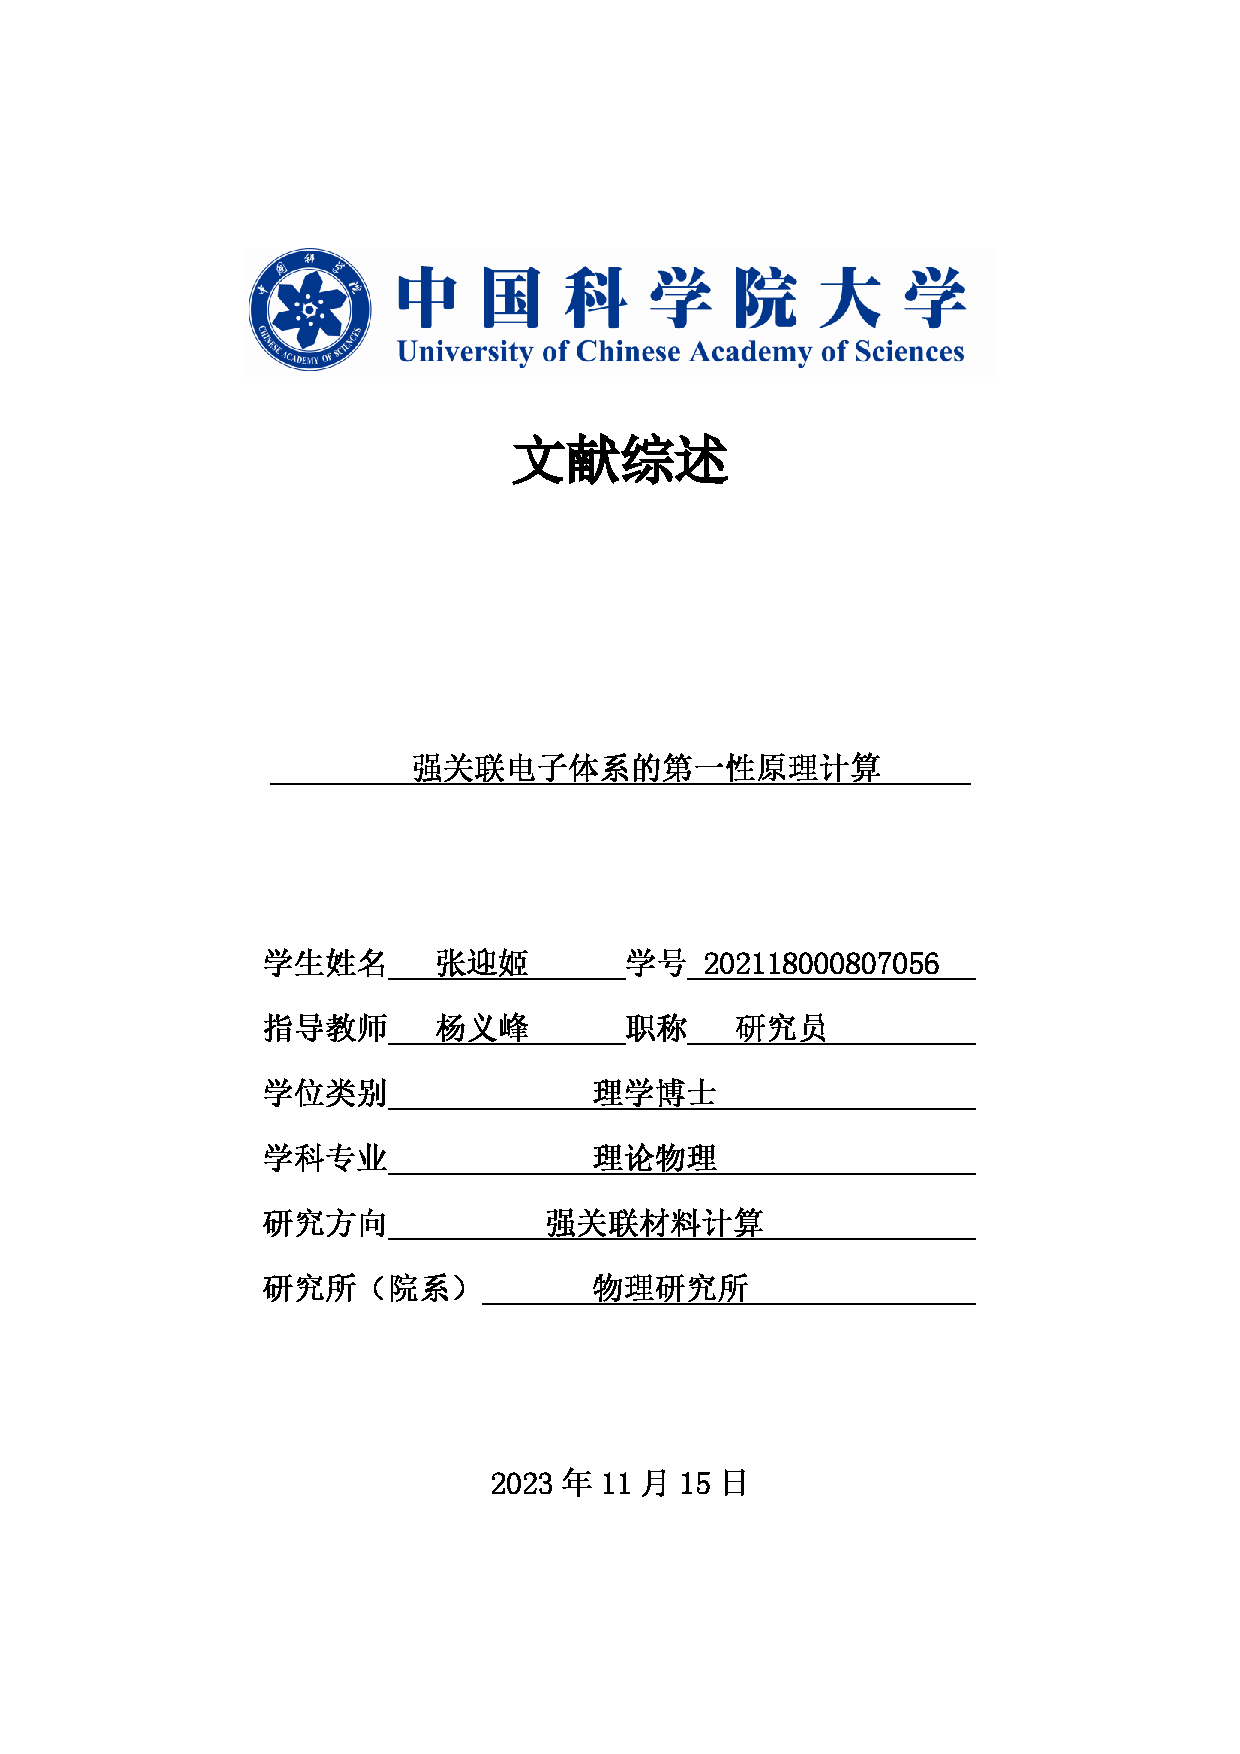
\includepdf{Img/Frontpage.pdf}
%-
%-> 中文摘要
%-
\intobmk\chapter*{摘\quad 要}% 显示在书签但不显示在目录
\setcounter{page}{1}% 开始页码
\pagenumbering{Roman}% 页码符号

在强关联材料计算中,电子关联会导致实际数值计算中遇到所谓的“指数墙”困难。为克服这一问题,人们不断发展了各种近似计算方案,从量子力学发展之初建立起的波恩-奥本海默近似,哈特利-福克近似,到后来成为主流计算方案的密度泛函理论,第一性原理计算的性能得到了不断提升。密度泛函理论的主要思路是体系全部物理性质都能够由基态密度唯一确定下来。这一方案的主要问题是囿于平均场图像,难以引入电子关联。为处理这一问题,人们进一步采用引入静态相互作用的 LDA+$U$ 方法来处理关联效应导致的电子局域化等性质,以及引入动态修正的 DFT+DMFT 方案,从而能够在实际计算中得到近藤物理相关性质。

\keywords{第一性原理计算,密度泛函理论,动力学平均场理论}% 中文关键词
%-
%-> 英文摘要
%-
\intobmk\chapter*{Abstract}% 显示在书签但不显示在目录

In strongly correlated material calculations, electronic correlations can lead to difficulties in obtaining accurate numerical results, commonly known as the "exponential wall" problem. To overcome this issue, various approximate computational schemes have been developed over time. These include the Born-Oppenheimer approximation and the Hartree-Fock approximation, which were established in the early stages of quantum mechanics, as well as the density functional theory (DFT), which has become the mainstream computational approach. The performance of first-principles calculations has been continuously improved. The main idea behind the density functional theory is that all physical properties of a system can be uniquely determined by its ground-state density. However, this approach is limited by the mean-field approximation and struggles to incorporate electronic correlations. To address this problem, researchers have introduced methods such as the LDA+U approach, which introduces static interaction to capture localized electronic properties affected by correlation effects, and the DFT+DMFT scheme, which incorporates dynamic corrections. These methods allow for the calculation of Kondo physics-related properties in practical computations.
    %- the current style, comment all the lines in plain style definition.

\KEYWORDS{First Principle Calculation, Density Functional Theory, Dynamical Mean Field Theory}% 英文关键词

\pagestyle{enfrontmatterstyle}%
\cleardoublepage\pagestyle{frontmatterstyle}%

%---------------------------------------------------------------------------%
